\section{Learning with SGD}
\frame{\tableofcontents[currentsection, hideothersubsections]}

\begin{frame}
\frametitle{Learning with SGD: Risk Minimization}

Recall, in learning:\\
\begin{itemize}
\item want to minimize the risk function, $L_D(\mathbf{w}) = \mathbb{E}_{z \approx D} [\ell(\mathbf{w}, z)]$
\item do not know $D$, so cannot simply calculate $L_D (w(t))$
\end{itemize}
\vspace{5mm}

With SGD:\\
find an unbiased estimate of the gradient of $L_D(\mathbf{w})$, that is,\\
a random vector whose conditional expected value is $L_D (\mathbf{w}^{(t)} )$

\end{frame}


\begin{frame}
\frametitle{Learning with SGD: Risk Minimization}

Construction of the random vector $v_t$ for  a differentiable risk fn $L_D$:
\begin{itemize}
\item sample $z \approx D$
\item define $v_t$ to be the gradient of the function $\ell(\mathbf{w}, z)$ wrt $\mathbf{w}$, at $\mathbf{w}^{(t)}$
\item by the linearity of the gradient we have:
    \begin{figure}
        \centering
        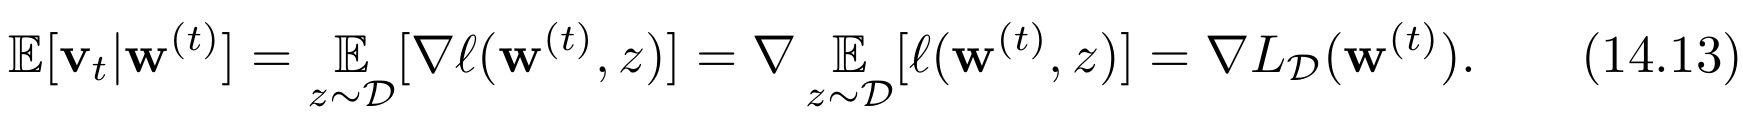
\includegraphics[scale=0.25]{eq_14_13}
    \end{figure}
\end{itemize}
\vspace{5mm}

Thus, the gradient of the loss function $\ell(w, z)$ at $\mathbf{w}^{(t)}$ is
\begin{itemize}
\item unbiased estimate of the gradient of the risk function $L_D( w^{(t)} )$ and
\item easily constructed by sampling a single fresh example $z \approx D$ at each iteration $t$.
\end{itemize}

\end{frame}


\begin{frame}
\frametitle{Learning with SGD: Risk Minimization}

\begin{figure}
    \centering
    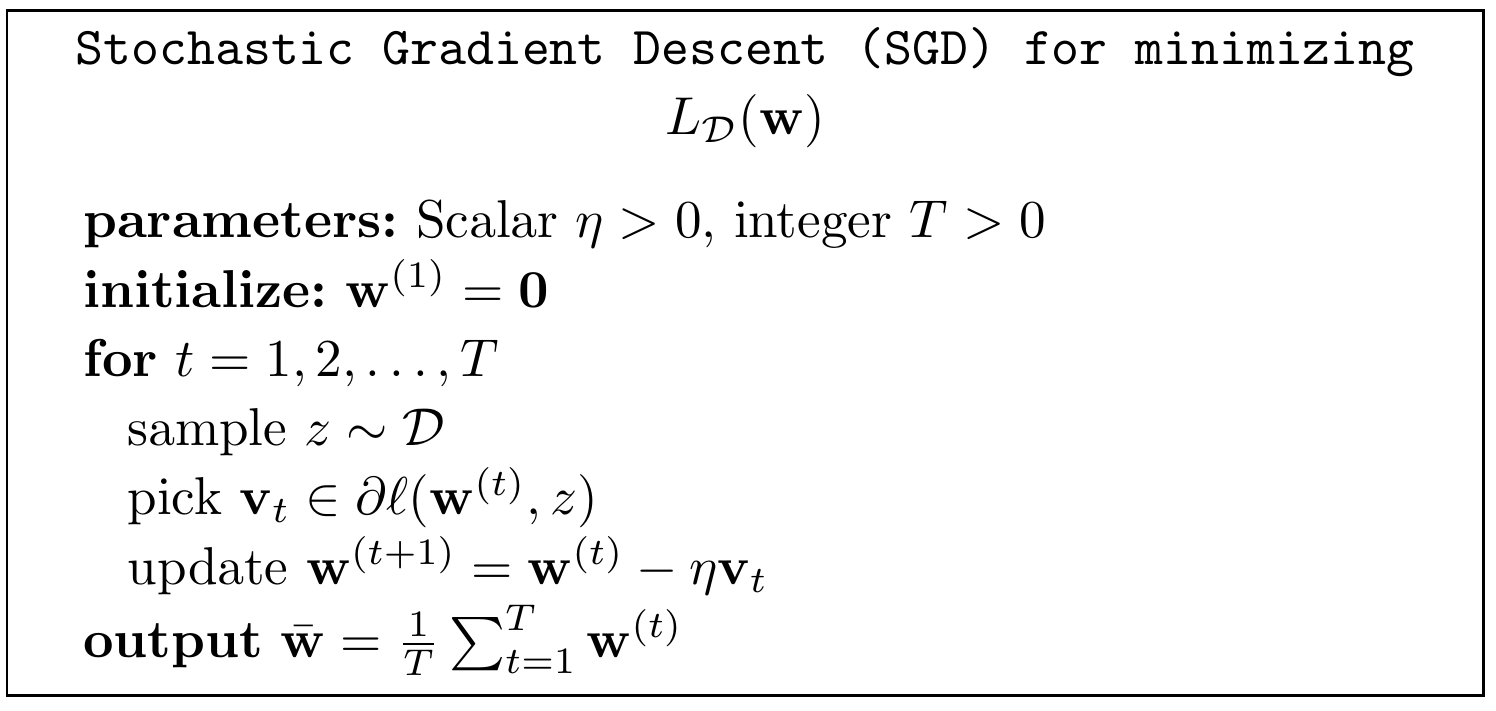
\includegraphics[scale=0.25]{sgd2}
\end{figure}

Same for nondifferentiable loss functions,\\
simply let $\mathbf{v}_t$ be a subgradient of $\ell(\mathbf{w}, z)$ at $\mathbf{w}^{(t)}$

\end{frame}

\begin{frame}
\frametitle{Learning with SGD: Convex-Smooth Learning Problems}

\begin{figure}
    \centering
    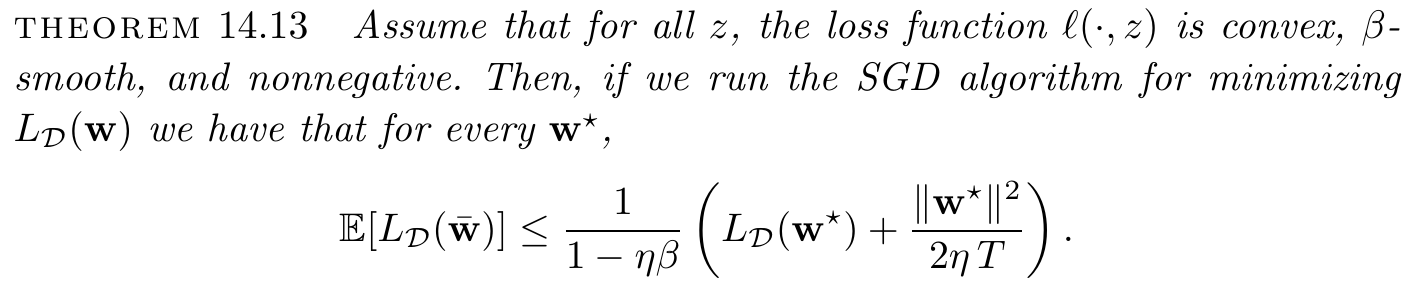
\includegraphics[scale=0.25]{theorem_14_13}
\end{figure}

\begin{figure}
    \centering
    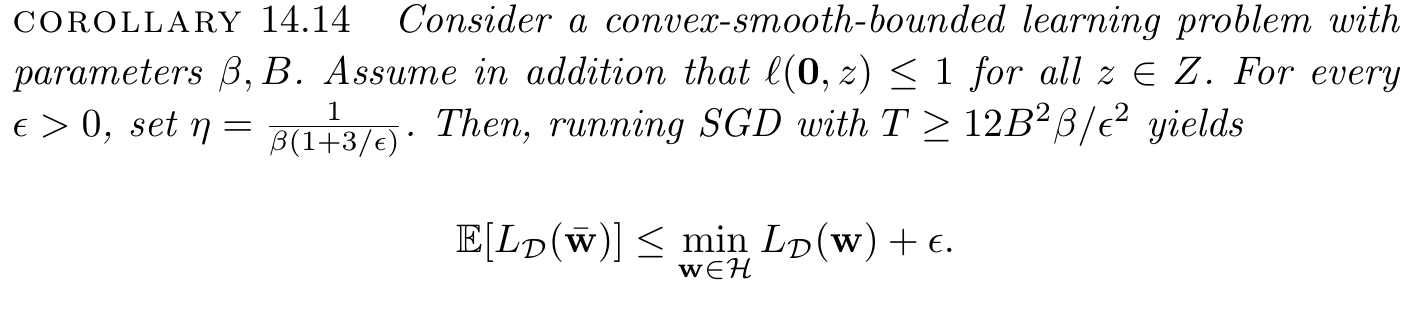
\includegraphics[scale=0.25]{corollary_14_14}
\end{figure}

\end{frame}

\begin{frame}
\frametitle{Learning with SGD: Regularized Loss Minimization}

WHAT:\\
to solve the regularized loss minimization:
\begin{figure}
    \centering
    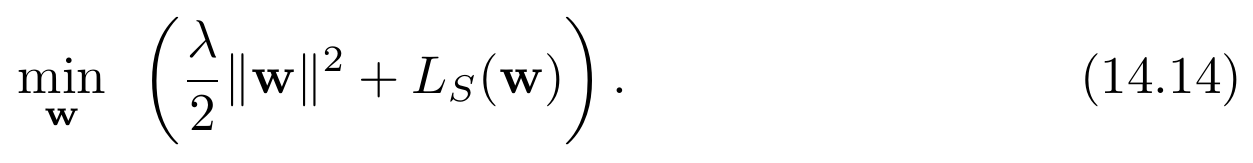
\includegraphics[scale=0.25]{eq_14_14}
\end{figure}

WHY:\\
\begin{itemize}
\item SGD enjoys the same worst-case sample complexity bound as regularized loss minimization
\item on some distributions, regularized loss minimization may yield a better solution.
\end{itemize}

HOW:\\
...
\end{frame}

\begin{frame}
\frametitle{Learning with SGD: Regularized Loss Minimization}

WHAT:\\
to solve the regularized loss minimization:
\begin{figure}
    \centering
    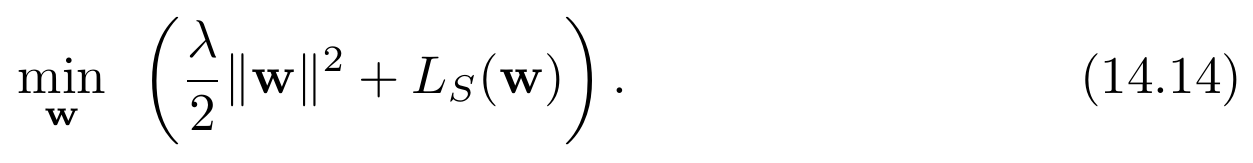
\includegraphics[scale=0.25]{eq_14_14}
\end{figure}

HOW:\\
\begin{itemize}
\item define $f(\mathbf{w}) = \frac{\lambda}{2} \parallel w \parallel^2 + L_S(\mathbf{w})$.
    \begin{itemize}
        \item $f$ is a $\lambda$-strongly convex function;
        \item therefore, apply the SGD variant with $\mathcal{H} = \mathbb{R}^d$.
    \end{itemize}
\item construct an unbiased estimate of a subgradient of $f$ at $\mathbf{w}^{(t)}$
    \begin{itemize}
        \item pick $z$ uniformly at random from $S$,
        \item choose $\mathbf{v}_t$ in $\partial \ell(\mathbf{w}^{(t)}, z)$
        \item (then) the expected value of $\lambda \mathbf{w}^{(t)} + \mathbf{v}t$ is a subgradient of f at $\mathbf{w}^{(t)}$.
    \end{itemize}
\end{itemize}

\end{frame}

